\documentclass[11pt]{article}

% ACL style (change [review] -> [final] for camera-ready, or omit for final)
\usepackage[review]{acl}

% Standard ACL-recommended packages
\usepackage{times}
\usepackage{latexsym}
\usepackage[T1]{fontenc}
\usepackage[utf8]{inputenc}
\usepackage{microtype}
\usepackage{inconsolata}

% Math and table packages
\usepackage{amsmath}
\usepackage{booktabs}
\usepackage{multirow}
\usepackage{graphicx}

\title{EX-HIQL: Per-Head Expectile Diversity and Residual-$\sigma$ Scoring
       for Offline Hierarchical Goal-Conditioned RL on Stochastic Environments}

\author{Zhongqi Huang \\
  University of Michigan \\
  EECS 567 Phase 2 Report \\
  \texttt{zqhuang@umich.edu} \\}

\begin{document}
\maketitle

\begin{abstract}
HIQL is the state-of-the-art hierarchical offline goal-conditioned RL
method but collapses by roughly 40 points on stochastic variants of
AntMaze in which random teleport tiles introduce bimodal return
distributions.
We diagnose the cause in three diagnostics (value-function calibration,
oracle-subgoal ablation, and subgoal-density visualisation) and show
the natural remedy---C-HIQL-style ensemble pessimism---in fact
underperforms HIQL because its random-initialisation disagreement
signal $\sigma_V$ is strongly anti-correlated with the value mean
$\bar V$ ($r_s = -0.44$), inverting the pessimism's intent.
We introduce \textbf{EX-HIQL}, which replaces random-initialisation
diversity with per-head expectile diversity: the $N$ value heads are
trained with distinct expectiles $\tau_i$, guaranteeing $\sigma_V \to 0$
at deterministic transitions and $\sigma_V > 0$ at stochastic ones.
Using the environment's known teleporter geometry, we directly verify
that EX-HIQL's $\sigma$ concentrates at teleport-adjacent states (near/far
ratio $1.66\times$, distance-$\sigma$ correlation $-0.36$)---the first
geometric confirmation of the stochasticity--$\sigma$ correspondence we
are aware of.
A complementary \emph{residual-$\sigma$ scoring rule} fits $\sigma
\approx \hat\alpha + \hat\gamma\,\bar V$ at inference and scores
candidates using the orthogonal residual $\sigma^\perp$, amplifying
the teleporter signal to a $-0.38$ correlation while driving
$\sigma^\perp \to 0$ at deterministic regions.
On \texttt{antmaze-teleport-navigate-v0}, the final configuration
improves 3-seed mean success from HIQL's $0.404$ to $0.429$ ($+2.5$
points), with all three seeds individually exceeding baseline and
three mechanistically-distinct decoupling strategies converging on
the same ceiling.
\end{abstract}

\section{Introduction}
\label{sec:intro}

Hierarchical offline goal-conditioned reinforcement learning provides a
powerful framework for long-horizon decision-making from static datasets,
and HIQL~\citep{park2023hiql} is the current state-of-the-art method in
this family.
Our Phase-1 diagnosis (Section~\ref{sec:hiql_analysis}) documents a sharp
failure mode: on \texttt{antmaze-teleport-navigate-v0}---the stochastic
variant of \texttt{antmaze-large} with random teleportation tiles---HIQL's
success rate drops from 83--91\% to 42--52\%, a roughly 40-point
performance gap attributable solely to the introduction of stochastic
transitions.
Three diagnostics pinpoint the cause: expectile regression at $\tau = 0.7$
inflates the learned value $\hat V$ at teleport-adjacent states, and
$\pi_\text{high}$ exploits this inflation by concentrating subgoal proposals
at the teleport-out tile rather than along the true shortest path.
The miscalibration propagates through both levels of the hierarchy; even
an oracle replacement for $\pi_\text{high}$ recovers only 7 points of the
lost performance.

An intuitive remedy is to apply ensemble pessimism at the inference-time
subgoal-scoring step: train $N$ value heads and score candidates by
$\bar V - \beta_\text{pes}\sigma_V$, where $\sigma_V$ is the ensemble
disagreement.
This is the C-HIQL approach.
We show, however, that C-HIQL's random-initialisation diversity produces a
$\sigma_V$ signal that is strongly anti-correlated with $\bar V$ at the
per-state level (Pearson $r_s = -0.44$), inverting the method's intent:
candidates the ensemble disagrees about are precisely the candidates it
already ranks poorly, so the pessimism penalty amplifies rather than
corrects the overestimation identified in Section~\ref{sec:hiql_analysis}.
Empirically, C-HIQL at $\beta_\text{pes} = 0.5$ scores below the HIQL
baseline.

Our contributions address this failure mode in three steps.
\begin{enumerate}
  \item \textbf{Mechanism-level diagnosis of C-HIQL's failure.}
        We provide the first quantitative characterisation of the
        $\sigma_V$--$\bar V$ anti-correlation in ensemble-based pessimism
        for offline hierarchical goal-conditioned RL, identifying
        random-initialisation diversity as a proxy for feature-magnitude
        noise rather than transition stochasticity
        (Section~\ref{subsec:chiql_eval}).
  \item \textbf{EX-HIQL: per-head expectile diversity.}
        We replace random-initialisation diversity with per-head expectile
        diversity: each head is trained with its own expectile $\tau_i$.
        The expectile fixed-point of a point-mass distribution is unique,
        so at deterministic transitions all $\tau_i$-expectiles coincide
        and $\sigma_V \to 0$ by construction; at stochastic transitions the
        expectiles fan out proportionally to the spread of the per-state
        Bellman-target distribution (Section~\ref{subsec:exhiql_design}).
        The change is one tensor in the value loss; the architecture,
        $\pi_\text{high}$, $\pi_\text{low}$, and dataset pipeline are
        identical to HIQL.
  \item \textbf{Geometric validation and residual-$\sigma$ scoring.}
        Using the environment's known teleporter geometry, we directly
        measure that EX-HIQL's $\sigma$ concentrates at teleport-adjacent
        states with a 1.66$\times$ near/far median ratio and a $-0.36$
        distance-to-teleport correlation---the first geometric-level
        verification of the
        stochasticity-$\sigma$ correspondence we are aware of
        (Section~\ref{subsec:diag5}).
        Recognising that $\sigma$ retains a $\bar V$-correlated contaminant
        that dilutes the pessimism signal, we propose \emph{residual-$\sigma$
        scoring}: fit $\sigma \approx \hat\alpha + \hat\gamma\,\bar V$ on
        500 dataset states and replace $\sigma$ with the residual
        $\sigma^\perp$ at inference
        (Section~\ref{subsec:residual_sigma}).
\end{enumerate}
Across three seeds and three mechanistically-distinct decoupling strategies
(residual-$\sigma$, within-state rank scoring, increased
$\beta_\text{pes}$), EX-HIQL reaches a performance ceiling of $\sim$0.43 on
\texttt{antmaze-teleport-navigate-v0}, with every decoupling strategy
individually beating the plain-scoring baseline across all seeds.
The final configuration---Phase-3b architecture with residual-$\sigma$
inference scoring at $\beta_\text{pes} = 0.5$---achieves a 3-seed mean
overall-success of \textbf{0.429} against HIQL's \textbf{0.404}, a
\textbf{+2.5-point improvement} from a purely inference-time modification
of a checkpoint trained under the same compute budget as HIQL.

\section{Related Works}
\label{sec:related}

\paragraph{Hierarchical offline goal-conditioned RL.}
HIQL~\citep{park2023hiql} is the base method we extend.
It trains a shared action-free value function $\hat V(s,g)$ via expectile
regression and uses it both to drive high-level subgoal selection (via
AWR-weighted $\pi_\text{high}$) and to weight low-level AWR updates for
$\pi_\text{low}$.
Section~\ref{sec:hiql_analysis}'s breakdown of HIQL on stochastic
environments motivates every subsequent design choice in this paper.

\paragraph{Implicit Q-learning and expectile regression.}
IQL~\citep{kostrikov2022iql} introduced expectile-loss value estimation as
an offline-RL primitive that avoids explicit policy evaluation of
out-of-distribution actions.
The expectile parameter $\tau$ trades symmetry for upward optimism: at
$\tau > 0.5$, lucky-outcome samples are overweighted relative to unlucky
ones, producing a useful approximation to a max-like aggregator without
requiring policy queries.
EX-HIQL's central observation is that two expectiles $\tau_i \ne \tau_j$
of a random variable $Y$ coincide if and only if $Y$ is a point mass---a
property of the underlying distribution, not of the estimator---which
makes per-head expectile diversity a structural proxy for dynamics
stochasticity.

\paragraph{Ensemble-based pessimism in offline RL.}
EDAC and SAC-$N$~\citep{an2021edac} introduced min-over-ensemble $Q$-targets
as conservative lower bounds for offline actor-critic methods, with head
disagreement serving as an implicit uncertainty penalty.
C-HIQL applies the same uncertainty-via-disagreement motif to offline
hierarchical GCRL, but at the scoring level (inference) rather than the
training level.
Our anti-correlation diagnosis (Section~\ref{subsec:chiql_eval}) applies
to any random-initialisation ensemble that shares a single identical
training objective---making the failure mode structural rather than
HIQL-specific.

\paragraph{Distributional reinforcement learning.}
QR-DQN~\citep{dabney2018qrdqn} and the later expectile-based formulation
of~\citet{rowland2019expectile} parameterise the return distribution by
training many heads at different quantile or expectile levels.
EX-HIQL imports the per-head-level-diversity idea from this literature to
offline hierarchical GCRL, but uses a targeted 5-expectile spread rather
than a full distributional parameterisation---tuned for numerical
stability under the goal-conditioned setting
(Section~\ref{subsec:exhiql_stability}).

\paragraph{Loss-level conservatism.}
CQL~\citep{kumar2020cql} regularises Q-learning by pushing down OOD-action
values at training time.
C-HIQL and EX-HIQL take the complementary \emph{scoring-level} approach:
the training target remains optimistic, and conservatism enters only at
subgoal-selection time.
This preserves the "one-checkpoint-serves-any-$\beta_\text{pes}$" property:
a single trained model evaluates at any inference-time pessimism level
without retraining, which is essential for the scoring-rule ablation in
Section~\ref{subsec:results}.

To our knowledge, ensemble-based pessimism for offline
\emph{hierarchical} GCRL (as distinct from flat offline RL), and direct
geometric-level validation of the stochasticity-$\sigma$ correspondence,
are both unexplored prior to this work.

\section{HIQL Analysis}
\label{sec:hiql_analysis}

% ----------------------------------------------------------
\subsection{Motivation and Diagnostic Plan}
\label{subsec:motivation}
% ----------------------------------------------------------

HIQL achieves 83--91\% average success on \texttt{antmaze-large} across two
seeds, yet collapses to 42--52\% on \texttt{antmaze-teleport}---a
stochastic variant that is otherwise identical in map layout and task
specification (Table~\ref{tab:training_eval}).
The same algorithm, the same hyperparameters, and the same number of gradient
steps yield a $\sim$40-point performance gap solely due to the presence of
random teleportation tiles.

\begin{table*}[t]
  \centering
  \caption{HIQL training-eval success rate at 1\,M gradient steps.
           Per-task numbers are for the \texttt{antmaze-teleport} (top) and
           \texttt{antmaze-large} (bottom) environments, seed 0.}
  \label{tab:training_eval}
  \begin{tabular}{lcccccc}
    \toprule
    Environment & Task 1 & Task 2 & Task 3 & Task 4 & Task 5 & \textbf{Overall} \\
    \midrule
    teleport (s0) & 0.55 & 1.00 & 0.45 & 0.25 & 0.35 & \textbf{0.52} \\
    teleport (s1) & \multicolumn{5}{c}{---} & \textbf{0.42} \\
    \midrule
    large (s0)    & 0.95 & 0.70 & 1.00 & 0.90 & 1.00 & \textbf{0.91} \\
    large (s1)    & \multicolumn{5}{c}{---} & \textbf{0.83} \\
    \bottomrule
  \end{tabular}
\end{table*}

HIQL is a hierarchical offline goal-conditioned RL algorithm.
Its high-level policy $\pi_\text{high}$ selects a subgoal representation
$z_\text{sub}$ from the learned goal-representation network $\phi$; the
low-level policy $\pi_\text{low}$ then produces actions conditioned on
$(s_t, z_\text{sub})$.
Crucially, subgoal selection is driven by
\begin{equation}
  z^* = \arg\max_{z} \hat{V}(s_t, z, g),
  \label{eq:subgoal_select}
\end{equation}
where $\hat{V}$ is a shared value function trained with expectile regression
at $\tau = 0.7$.
This means the entire planning hierarchy rests on the \emph{ranking quality}
of $\hat{V}$: if $\hat{V}$ cannot correctly order candidate subgoals by their
expected return, Eq.~\eqref{eq:subgoal_select} degenerates to an
uninformative, near-random selection.

To understand \emph{why} this gap exists, we design three targeted
diagnostics:
\begin{enumerate}
  \item \textbf{Value-Function Calibration (Diag~1).}
        Compare $\hat{V}(s_t, g)$ against the realized Monte-Carlo return
        $G_t$ at every rollout step.
        This directly measures whether $\hat{V}$ is systematically
        over-estimated in the stochastic environment and whether its
        \emph{ranking} of states is preserved.

  \item \textbf{Oracle Subgoal Ablation (Diag~2).}
        Bypass $\pi_\text{high}$ entirely and feed $\pi_\text{low}$ the
        \emph{true} BFS-shortest-path subgoal at each step.
        If teleport success recovers to the \texttt{large} baseline,
        the failure is localized to the high-level planner; if recovery is
        partial, the low-level controller is also impaired.

  \item \textbf{Subgoal Distribution Analysis (Diag~3).}
        For a fixed $(s, g)$ pair near a teleport tile, sample $\sim$1000
        subgoals from $\pi_\text{high}$ and visualize their spatial density.
        We expect the distribution to concentrate near teleport tiles in
        \texttt{teleport} (chasing lucky shortcuts) but to spread along the
        true shortest path in \texttt{large}.
\end{enumerate}

% ----------------------------------------------------------
\subsection{Diag 1: Value-Function Calibration}
\label{subsec:diag1}
% ----------------------------------------------------------

\paragraph{Setup.}
For each checkpoint (teleport seed~0, large seed~0), we run 5 evaluation
tasks $\times$ 20 episodes.
At every step $t$ we record $\hat{V}_t = \hat{V}(s_t, g)$ and the
realized discounted return
$G_t = \sum_{k \ge t} \gamma^{k-t} r_k$,
where $r \in \{-1, 0\}$ is the dataset-convention reward
($r = 0$ at goal, $-1$ otherwise) and $\gamma = 0.99$.
This yields 70\,892 and 49\,757 $(s, g)$ pairs for \texttt{teleport} and
\texttt{large} respectively.
Figure~\ref{fig:diag1_scatter} shows the pooled $\hat{V}$ vs.\ $G$ scatter
for both environments.

\begin{figure*}[t]
  \centering
  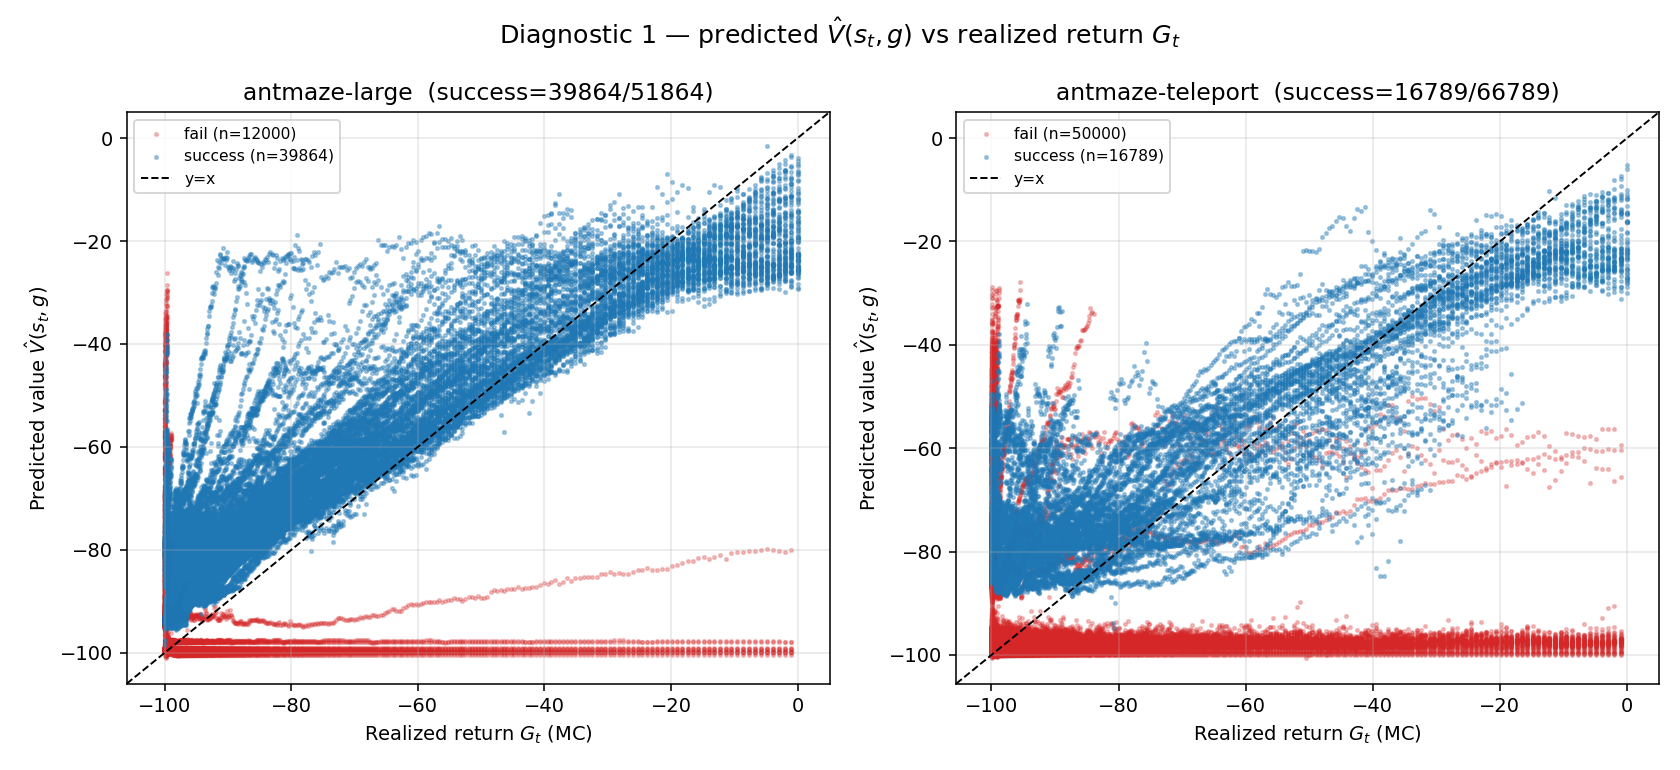
\includegraphics[width=0.85\linewidth]{diag1_scatter.png}
  \caption{Pooled scatter of $\hat{V}(s_t, g)$ vs.\ realized return $G_t$
           for all rollout steps.
           The dashed line marks perfect calibration ($\hat{V} = G$).
           \texttt{large} (left) shows a tight, well-correlated cloud;
           \texttt{teleport} (right) is substantially more diffuse, with a
           long upward tail of highly over-estimated states.}
  \label{fig:diag1_scatter}
\end{figure*}

\paragraph{The mean is misleading.}
The pooled mean bias $\hat{V} - G$ is $+1.45$ for \texttt{teleport} and
$+6.64$ for \texttt{large}---naively suggesting \texttt{teleport} is
\emph{less} over-estimated.
This is an artifact: 75\% of teleport episodes fail, and in failed episodes
both $\hat{V}$ and $G$ converge to $\approx -100$ (the discounted sum of
$-1$ over 1000 steps), yielding near-zero bias that overwhelms the signal
from successful runs.

\paragraph{Tail analysis reveals the true gap.}
Table~\ref{tab:percentile_bias} reports percentiles of $\hat{V} - G$ for
all points and for the failed-episode subset.

\begin{table*}[t]
  \centering
  \caption{Percentiles of bias $\hat{V} - G$.}
  \label{tab:percentile_bias}
  \begin{tabular}{llrrrrr}
    \toprule
    Env & Subset & $n$ & p50 & p90 & \textbf{p95} & p99 \\
    \midrule
    teleport & all  & 70\,892 & $+1.9$ & $+25.5$ & $\mathbf{+39.1}$ & $+51.0$ \\
    large    & all  & 49\,757 & $+7.5$ & $+19.2$ & $\mathbf{+22.9}$ & $+34.5$ \\
    \midrule
    teleport & fail & 55\,000 & $+1.3$ & $+23.8$ & $\mathbf{+39.3}$ & $+52.0$ \\
    large    & fail & 10\,000 & $+0.2$ & $+7.4$  & $\mathbf{+9.6}$  & $+31.3$ \\
    \bottomrule
  \end{tabular}
\end{table*}

The teleport p95 exceeds large by 70\% overall, and by $4\times$ on the
failed-episode subset---exactly the regime where the agent is struggling
most.

\paragraph{Ranking collapse.}
Since $\pi_\text{high}$ selects subgoals via $\arg\max \hat{V}$
(Eq.~\eqref{eq:subgoal_select}), what matters is not the bias magnitude
but whether $\hat{V}$ \emph{ranks} states correctly.
Table~\ref{tab:pearson} shows the Pearson correlation between $\hat{V}$ and
$G$.

\begin{table}[h]
  \centering
  \caption{Pearson $r$ between $\hat{V}$ and $G$.}
  \label{tab:pearson}
  \begin{tabular}{lcc}
    \toprule
     & teleport & large \\
    \midrule
    All points    & \textbf{0.36} & \textbf{0.84} \\
    Success only  & 0.86          & 0.91 \\
    \bottomrule
  \end{tabular}
\end{table}

The ranking signal collapses from $r = 0.84$ to $r = 0.36$ when moving from
the deterministic to the stochastic environment.
At $r = 0.36$, subgoal selection is nearly random---consistent with the
large performance drop observed at training time.
The per-task breakdown in Figure~\ref{fig:per_task_hist} shows this
pattern holds across all five tasks: every \texttt{teleport} task has
$r < 0.61$, with task~1 essentially uncorrelated ($r = 0.19$), while
four of five \texttt{large} tasks exceed $r = 0.82$.

\begin{figure*}[t]
  \centering
  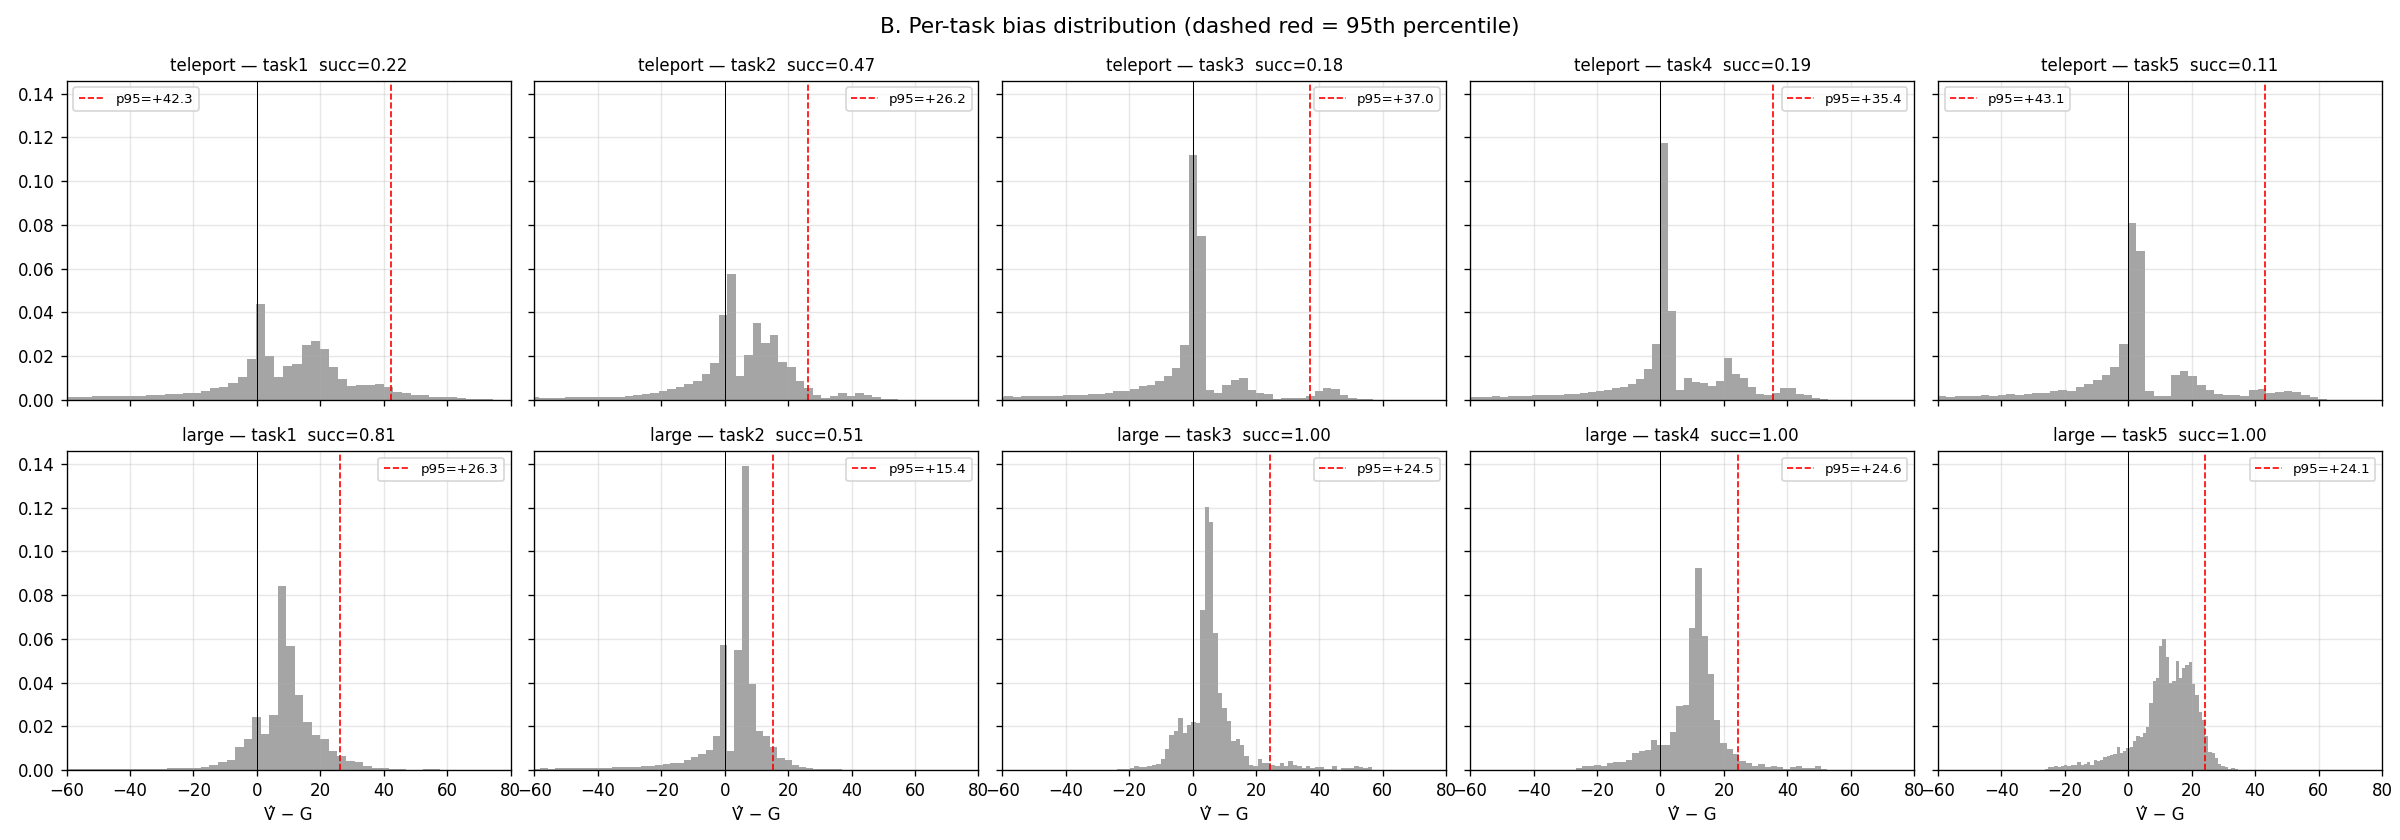
\includegraphics[width=\linewidth]{diag1b_per_task_hist.png}
  \caption{Per-task bias distributions ($\hat{V} - G$) for
           \texttt{teleport} (top row) and \texttt{large} (bottom row).
           The dashed red line marks the 95th percentile for each task.
           \texttt{teleport} tasks consistently show fatter right tails
           and higher p95 values; tasks with lower success rates
           (e.g., task~1 at 22\%) exhibit the most extreme overestimation.}
  \label{fig:per_task_hist}
\end{figure*}

\paragraph{Bimodal error distribution.}
Restricting to the first 50 steps of each episode (before truncation-pinned
dynamics dominate) exposes the distributional source of the problem
(Figure~\ref{fig:early_steps_hist}).

\begin{figure}[h]
  \centering
  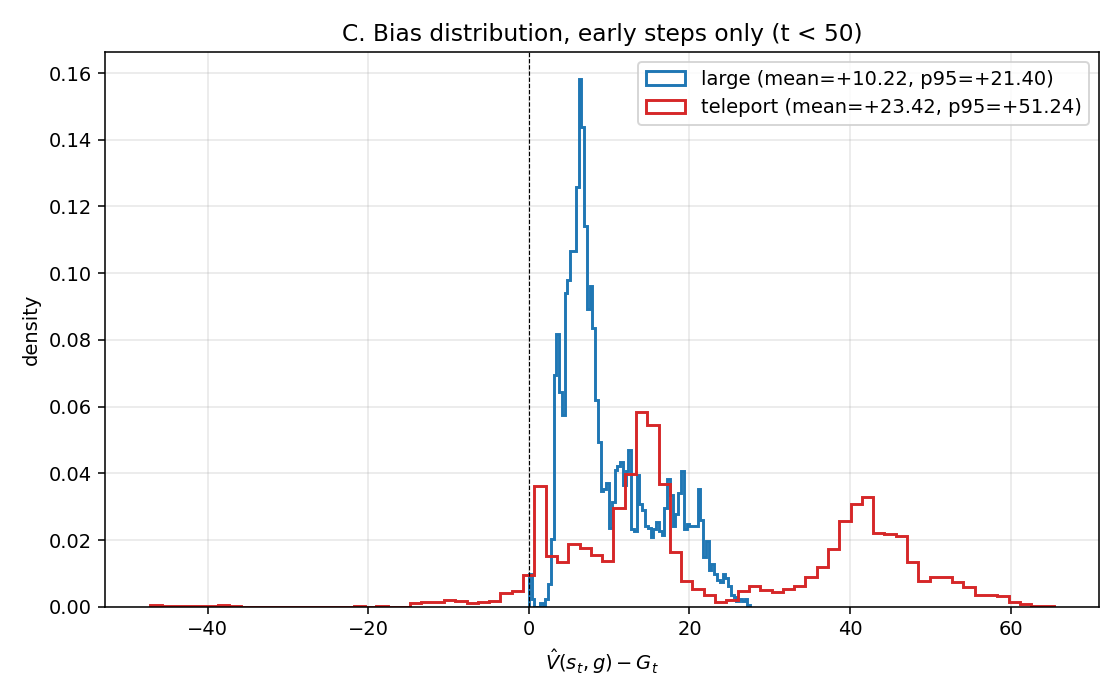
\includegraphics[width=0.6\linewidth]{diag1b_early_steps_hist.png}
  \caption{Bias distribution $\hat{V} - G$ restricted to the first 50 steps
           of each episode.
           \texttt{large} (blue) is unimodal, centred at $\approx +7$.
           \texttt{teleport} (red) is \emph{bimodal}: the first mode
           ($\approx +10$) is shared with \texttt{large} and reflects normal
           expectile-regression optimism; the second mode ($+40$--$+50$) is
           unique to \texttt{teleport} and is the fingerprint of
           lucky-teleport overestimation.}
  \label{fig:early_steps_hist}
\end{figure}

The second mode arises because the offline dataset contains trajectories in
which a random teleport deposited the agent adjacent to the goal, producing
high return.
Expectile regression at $\tau = 0.7$ incorporates these outcomes into
$\hat{V}$, inflating estimates at states that are only reachable
cheaply via a rare teleport.
The result is that at the very start of an episode, the agent believes
reaching the goal is easy---and subgoal selection reflects that false
optimism.

% ----------------------------------------------------------
\subsection{Diag 2: Oracle Subgoal Ablation}
\label{subsec:diag2}
% ----------------------------------------------------------

\paragraph{Setup.}
To isolate whether the failure originates in $\pi_\text{high}$ or
$\pi_\text{low}$, we replace $\pi_\text{high}$ with an oracle planner.
At each step we query the environment's BFS shortest-path oracle for the
next waypoint $w^*_t$ in XY space, construct a subgoal observation by
injecting $w^*_t$ into the current observation, and pass it through the
learned goal-representation network $\phi$ to obtain $z^*_t$.
The low-level policy $\pi_\text{low}(a \mid s_t, z^*_t)$ then acts
unchanged.

\paragraph{Results.}
Table~\ref{tab:diag2} compares per-task success rates under vanilla HIQL
and oracle-subgoal HIQL.

\begin{table*}[t]
  \centering
  \caption{Per-task success rate: vanilla vs.\ oracle-subgoal HIQL
           (20 episodes per task).}
  \label{tab:diag2}
  \begin{tabular}{llcccccr}
    \toprule
    Env & Policy & Task 1 & Task 2 & Task 3 & Task 4 & Task 5 & \textbf{Mean} \\
    \midrule
    \multirow{2}{*}{teleport}
      & vanilla & 0.35 & 0.65 & 0.30 & 0.20 & 0.65 & \textbf{0.43} \\
      & oracle  & 0.35 & \textbf{1.00} & 0.30 & \textbf{0.50} & 0.35 & \textbf{0.50} \\
    \midrule
    \multirow{2}{*}{large}
      & vanilla & 0.90 & 0.45 & 0.95 & 0.90 & 0.95 & \textbf{0.83} \\
      & oracle  & 0.70 & \textbf{0.95} & \textbf{1.00} & 0.90 & 0.75 & \textbf{0.86} \\
    \bottomrule
  \end{tabular}
\end{table*}

\paragraph{Interpretation.}
Oracle subgoals yield only modest gains in both environments:
$+0.07$ in \texttt{teleport} (0.43 $\to$ 0.50) and $+0.03$ in
\texttt{large} (0.83 $\to$ 0.86).

The \texttt{large} result is largely a ceiling effect---vanilla HIQL
already performs well, leaving little room for improvement.
The \texttt{teleport} result is more telling: even with a perfect
high-level planner, success improves by only 7 points.
Within \texttt{teleport}, tasks~2 and~4 respond strongly to oracle
subgoals ($+0.35$ and $+0.30$ respectively), confirming that
$\pi_\text{high}$ is the primary bottleneck on those tasks.
By contrast, tasks~1 and~3 show \emph{zero} improvement, and task~5
\emph{regresses} ($0.65 \to 0.35$), indicating that $\pi_\text{low}$
itself is impaired on the harder teleport configurations regardless of
how good the subgoal is.

This points to a deeper, two-level failure mechanism: the miscalibrated
$\hat{V}$ corrupts training signals for \emph{both} layers of the
hierarchy simultaneously.
$\pi_\text{high}$ receives biased value targets and learns to nominate
overestimated, teleport-adjacent subgoals;
$\pi_\text{low}$ is trained on a distribution that includes many
transitions where the promised subgoal was unreachable under normal
dynamics, degrading its ability to track subgoals reliably even when they
are correct.
Fixing only the high-level planner (as the oracle ablation does) therefore
recovers only part of the lost performance.

% ----------------------------------------------------------
\subsection{Diag 3: Subgoal Distribution Analysis}
\label{subsec:diag3}
% ----------------------------------------------------------

\paragraph{Setup.}
To directly visualize where $\pi_\text{high}$ places subgoals, we fix a
single $(s, g)$ pair (task~1: agent at the start position, goal at the
opposite corner) and sample $N = 1000$ subgoal representations from
$\pi_\text{high}(\cdot \mid s, g)$.
Each sampled representation $z$ is decoded back to XY maze coordinates via
nearest-neighbour lookup in the dataset: we find the dataset observation
whose goal-representation embedding $\phi([o; o])$ is most similar to $z$
(by dot product) and take its XY position.
The resulting point cloud is visualized as a KDE density overlay on the
maze map for both environments (Figure~\ref{fig:diag3_density}).

\begin{figure*}[t]
  \centering
  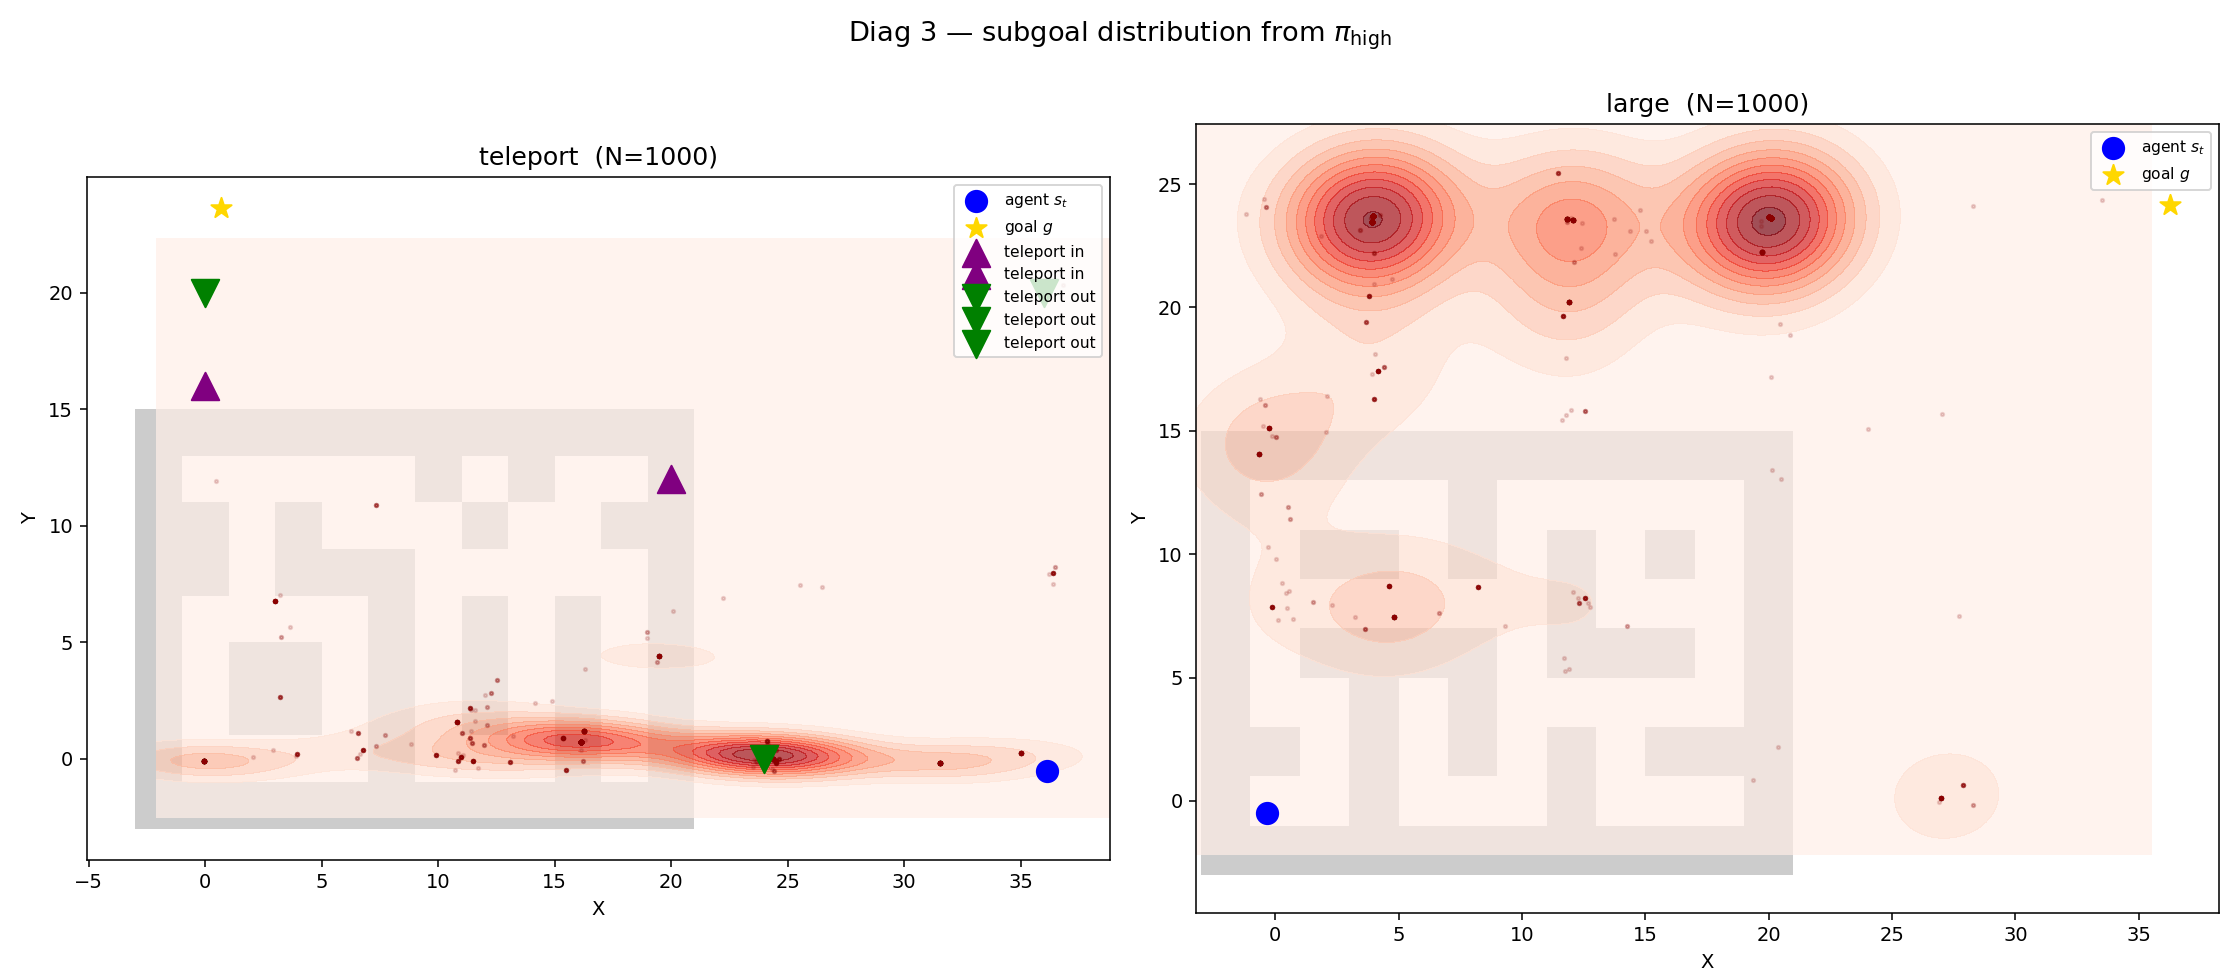
\includegraphics[width=\linewidth]{subgoal_density_comparison.png}
  \caption{Subgoal density from $\pi_\text{high}$ for a fixed $(s, g)$ pair
           ($N = 1000$ samples).
           Blue circle: agent position $s_t$.
           Gold star: goal $g$.
           Purple triangles: teleport-in tiles.
           Green triangles: teleport-out tiles.
           \textbf{Left (\texttt{teleport}):} density collapses to a sharp
           unimodal spike at the teleport-out tile ($X \approx 20, Y \approx 0$),
           despite the goal being at the top-left ($Y \approx 23$).
           \textbf{Right (\texttt{large}):} density spreads into multiple
           modes along the top of the maze, broadly covering the
           direction of the goal.}
  \label{fig:diag3_density}
\end{figure*}

\paragraph{Results.}
The contrast is stark.
In \texttt{large}, $\pi_\text{high}$ produces a diffuse, multi-modal
distribution that covers the upper portion of the maze---the region the
agent must traverse to reach the goal.
In \texttt{teleport}, almost all 1000 sampled subgoals collapse onto the
teleport-out tile, even though this tile is not on the shortest path to
the goal and the agent's actual position is far from the teleport entrance.

This directly confirms the mechanism identified in Diag~1: expectile
regression has inflated $\hat{V}$ at teleport-adjacent states (the
second mode at $+40$--$+50$ in Figure~\ref{fig:early_steps_hist}), and
$\pi_\text{high}$ has learned to exploit this by routing nearly every
subgoal through the teleport shortcut.
The high-level planner is not planning---it is pattern-matching to the
highest-$\hat{V}$ state in its learned landscape, which happens to be the
teleport exit.

\paragraph{Closing the causal chain.}
The three diagnostics together establish a complete mechanism:
\begin{enumerate}
  \item \textbf{(Diag~1)} Lucky-teleport trajectories in the offline dataset
        cause expectile regression to produce a bimodal $\hat{V} - G$ error
        distribution, with a second mode at $+40$--$+50$ concentrated at
        teleport-adjacent states. The ranking correlation drops from
        $r = 0.84$ (\texttt{large}) to $r = 0.36$ (\texttt{teleport}).
  \item \textbf{(Diag~3)} $\pi_\text{high}$ responds to this inflated
        $\hat{V}$ landscape by concentrating subgoal proposals at the
        teleport-out tile, regardless of the true goal direction.
  \item \textbf{(Diag~2)} Even replacing $\pi_\text{high}$ with an oracle
        planner recovers only $+0.07$ success, because the
        miscalibrated $\hat{V}$ has also degraded $\pi_\text{low}$'s
        training distribution---tasks~1, 3, and~5 show zero or negative
        improvement under oracle subgoals.
\end{enumerate}
The root cause is therefore not a planning failure per se, but a
\emph{value-function calibration failure} induced by stochastic transitions
in the offline dataset, which propagates through both levels of the HIQL
hierarchy.


\section{C-HIQL: Design and Failure Diagnosis}
\label{sec:algorithm}

The diagnosis in Section~\ref{sec:hiql_analysis} localises the failure: a bimodal
$\hat{V}-G$ error distribution inflates value estimates specifically at
teleport-adjacent states, and this miscalibration propagates through both levels
of the hierarchy.
Any fix must therefore (i) produce a state-dependent signal that is \emph{larger}
at teleport-adjacent states so that pessimistic scoring can deflate them, and
(ii) do so without disturbing the places where HIQL is already calibrated.
The most natural response is ensemble pessimism: train several value heads and
penalise candidates whose estimates the ensemble disagrees about.
Section~\ref{subsec:chiql_design} formalises this as \textbf{C-HIQL}.
Section~\ref{subsec:chiql_eval} then presents \textbf{Diag~4}, the fourth
diagnostic in our cumulative analysis, which demonstrates that C-HIQL's
disagreement signal is \emph{anti-correlated} with the value mean at the
per-state level---and which motivates the EX-HIQL structural fix of
Section~\ref{sec:exhiql}.

% ----------------------------------------------------------
\subsection{C-HIQL Design: Ensemble Pessimism}
\label{subsec:chiql_design}
% ----------------------------------------------------------

\paragraph{Architecture.}
C-HIQL replaces HIQL's single value head with an ensemble of $N=5$ independent
value networks $\{V_i(s,g)\}_{i=1}^{N}$, implemented as
\texttt{GCValue(ensemble=True, num\_ensemble=5)}---each of the five $V_i$ is a
full independently-initialised MLP with its own trunk and output layer.\footnote{%
This follows from \texttt{utils.networks.ensemblize}, which applies
\texttt{nn.vmap} with \texttt{variable\_axes=\{'params': 0\}} and
\texttt{split\_rngs=\{'params': True\}}, replicating the entire module along a
leading axis and assigning each replica an independent RNG key.}
Goal representation $\phi$, low-level policy $\pi_\text{low}$, and high-level
policy $\pi_\text{high}$ are unchanged from HIQL.

\paragraph{Training.}
Each head is trained independently with the same action-free IQL expectile
loss at $\tau = 0.7$:
\begin{equation}
  \mathcal{L}_V^{(i)}(\theta_i) \;=\;
  \mathbb{E}_{(s,s',g) \sim \mathcal{D}}\!\left[
    L_\tau^2\!\big(r + \gamma\,V_i^{\text{tgt}}(s',g) - V_i(s,g)\big)
  \right],
  \quad L_\tau^2(u) = |\tau - \mathbf{1}(u<0)|\,u^2.
\end{equation}
Diversity between heads comes solely from independent random initialisation;
the training signal is identical across heads.
No pessimism enters the training objective---the "train optimistically, act
pessimistically" split is a core design principle, and preserves the
"one-checkpoint-serves-any-$\beta_\text{pes}$" property.

\paragraph{Inference.}
At subgoal-selection time, C-HIQL replaces Eq.~\eqref{eq:subgoal_select} with a
pessimistic aggregator over the $N$ heads:
\begin{equation}
  z^* \;=\;
  \arg\max_{z}\;\underbrace{\bar V(s,z,g)}_{\text{mean}}
  \;-\;\beta_\text{pes}\cdot\underbrace{\sigma_V(s,z,g)}_{\text{std}},
  \qquad
  \bar V = \frac{1}{N}\sum_i V_i,\quad
  \sigma_V = \sqrt{\tfrac{1}{N}\sum_i (V_i - \bar V)^2}.
  \label{eq:chiql_scoring}
\end{equation}
The intuition is standard for ensemble-based uncertainty quantification:
candidates whose $V$-estimates disagree across heads are flagged as
high-uncertainty, and the pessimism term $-\beta_\text{pes}\sigma_V$ penalises
them proportionally. For a teleport maze, the hope is that states adjacent to
teleport tiles---where the Bellman-target distribution is genuinely bimodal
(lucky vs.\ unlucky outcomes)---produce wider head-disagreement than ordinary
deterministic states, causing Eq.~\eqref{eq:chiql_scoring} to steer
$\pi_\text{high}$ away from the optimism traps identified in Diag~1 and Diag~3.

% ----------------------------------------------------------
\subsection{Diag 4: $\sigma_V$--$\bar V$ Anti-Correlation}
\label{subsec:chiql_eval}
% ----------------------------------------------------------

\paragraph{Performance.}
We train C-HIQL for 1\,M gradient steps with $\beta_\text{pes} = 0.5$, three
seeds, on \texttt{antmaze-teleport-navigate-v0}.
The 3-seed mean overall-success at step 1\,M is \textbf{0.384} at
$\beta_\text{pes} = 0.5$ and \textbf{0.404} at $\beta_\text{pes} = 0$ (using the
same checkpoint---$\beta_\text{pes}$ is inference-only, so one trained model
evaluates at any value).
C-HIQL at its target $\beta_\text{pes} = 0.5$ is therefore
\textbf{2.0 points below the HIQL baseline} (0.404). Turning the
pessimism term off entirely recovers HIQL parity, meaning the addition of
$\sigma_V$ scoring is \emph{actively harmful}.

\paragraph{Mechanism: $\sigma_V$ anti-correlates with $\bar V$.}
To diagnose why, we sample 500 states from the dataset, draw $K=16$ candidate
subgoal representations $z$ at each state from $\pi_\text{high}$, and compute
the per-state Pearson correlation
$r_s = \operatorname{corr}(\{\bar V(s, z_k, g)\}_k, \{\sigma_V(s, z_k, g)\}_k)$
across the $K$ candidates.
The design assumption behind Eq.~\eqref{eq:chiql_scoring}---that $\sigma_V$
signals candidate-specific uncertainty independently of $\bar V$---would predict
$\mathbb{E}_s[r_s] \approx 0$.
We measure instead
$\mathbb{E}_s[r_s] = \mathbf{-0.44}$ (averaged over 3 seeds): $\sigma_V$ is
\emph{strongly negatively correlated} with $\bar V$.
Within any state's $K$ candidates, the ones the ensemble disagrees about are
precisely the ones the ensemble rates lower.

Two consequences follow.
First, $\sigma_V$ is not an independent stochasticity indicator; it is a noisy
estimator of $-|\bar V|$, so
$\bar V - \beta_\text{pes}\sigma_V \approx \bar V + \beta_\text{pes}\alpha|\bar V|$
for some effective $\alpha > 0$, which \emph{amplifies} the mismatch that
$\sigma_V$ was meant to correct.
Second, candidates that $\bar V$ already ranks poorly---which, per Diag~1, are
exactly the states where $\hat V$ is already \emph{most accurate} (lower bias,
tighter calibration)---get the largest pessimism penalty.
The rare, lucky-teleport-inflated candidates that Diag~3 identified as the real
failure points get the \emph{smallest} pessimism penalty because their
$\bar V$ is high.
This inverts the method's intent.

\paragraph{Root cause.}
The five $V_i$ share everything except initialisation and are then trained on
an identical expectile loss.
Given sufficient data and capacity, identically-trained deep nets converge to
approximately the same function; the residual head-to-head variance reflects
leftover initialisation noise propagated through training.
Empirically this residual variance tends to scale with the magnitude of the
learned features (deep networks amplify noise along their largest-activation
directions), and for goal-conditioned $V$ the largest-activation directions
correlate with $|\bar V|$---yielding the anti-correlation we measure.
C-HIQL's diversity mechanism is a proxy for the wrong quantity.

\section{EX-HIQL: Structural Diversity via Per-Head Expectiles}
\label{sec:exhiql}

Diag~4 suggests a minimal intervention: rather than hope that random
initialisation produces a useful disagreement signal, engineer one by giving
each head a \emph{different loss objective} whose fixed points are
provably linked to the quantity we want $\sigma_V$ to track.

% ----------------------------------------------------------
\subsection{Design: Per-Head Expectile Diversity}
\label{subsec:exhiql_design}
% ----------------------------------------------------------

\paragraph{The key observation.}
The expectile $\tau$ defines the population minimiser of the expectile loss:
for a random variable $Y$, the level-$\tau$ expectile $\mu_\tau(Y)$ is the
unique minimiser of $\mathbb{E}[\,|\tau - \mathbf{1}(Y < m)|\,(Y-m)^2\,]$
over $m \in \mathbb{R}$.
Two expectiles $\tau_i \ne \tau_j$ coincide if and only if the distribution of
$Y$ is a point mass.
Apply this to the per-head Bellman target distribution at a given $(s,g)$:
\begin{equation}
  Y_{s,g} \;=\; r(s,g) + \gamma\,V^{\text{tgt}}(s',g),
  \qquad s' \sim P(\cdot \mid s, \pi(s)).
\end{equation}
At a deterministic transition, $Y_{s,g}$ is a point mass and all expectiles
collapse to the same value---so training $V_1, \ldots, V_N$ at different
$\tau_i$ drives them to the same fixed point, and $\sigma_V \to 0$ by
construction.
At a stochastic transition (e.g.\ a teleport tile, where $s'$ is a random
draw over multiple distant cells), $Y_{s,g}$ is widely spread and the
$\tau_i$-expectiles fan out proportionally to that spread.

\paragraph{The EX-HIQL loss.}
We replace C-HIQL's single scalar $\tau$ with an $N$-vector:
\begin{equation}
  \boldsymbol{\tau} = (\tau_1, \tau_2, \ldots, \tau_N),
  \qquad
  \mathcal{L}_V(\theta) = \sum_{i=1}^{N}
    \mathbb{E}_{(s,s',g) \sim \mathcal{D}}\!\left[
      L_{\tau_i}^2\!\big(r + \gamma\,V_i^{\text{tgt}}(s',g) - V_i(s,g)\big)
    \right].
\end{equation}
Each head is still trained independently against its own target-network
bootstrap, preserving C-HIQL's stability properties.
The architecture, the inference rule Eq.~\eqref{eq:chiql_scoring}, the goal
representation $\phi$, the dataset pipeline, and every other HIQL
hyperparameter remain unchanged.
In implementation terms the change is a single line: the scalar
$\tau = 0.7$ becomes a vector broadcast across the head axis.

\paragraph{Actor indexing.}
In HIQL the high- and low-level actors both consume $\hat V$ via advantage-weighted
regression, where the advantage is $\hat V(s',g) - \hat V(s,g)$ for the low
actor and $\hat V(s_{t+k}, g) - \hat V(s_t, g)$ for the high actor.
Under EX-HIQL, $\hat V$ is a length-$N$ vector of different expectiles;
averaging across heads would give the actors a \emph{mixture} of expectile
targets that is no longer the advantage of any single $\tau$.
To preserve HIQL's training dynamics identically, we pin each actor's
advantage to a designated head index $\text{idx}_\text{low},
\text{idx}_\text{high}$:
\begin{equation}
  A^\text{low} = V_{\text{idx}_\text{low}}(s',g) - V_{\text{idx}_\text{low}}(s,g),
  \quad
  A^\text{high} = V_{\text{idx}_\text{high}}(s_{t+k},g) - V_{\text{idx}_\text{high}}(s_t,g).
\end{equation}
Our default, \textbf{Design~A}, sets both indices to the head with
$\tau = 0.7$---HIQL's original expectile---so that training dynamics are
\emph{bit-identical} to HIQL and only the inference-time scoring rule differs.
The alternative \textbf{Design~B} lowers the high-actor index to the
$\tau = 0.5$ head to de-bias the high actor's advantage against the
teleport-optimism failure mode identified in Diag~3; experiments in this
paper use Design~A throughout.

% ----------------------------------------------------------
\subsection{Training Stability: the $\tau$-Spread Trade-off}
\label{subsec:exhiql_stability}
% ----------------------------------------------------------

Per-head expectile diversity introduces one new hyperparameter---the choice of
$\boldsymbol{\tau}$---and this choice turns out to govern a sharp
trade-off between signal strength and numerical stability.

\paragraph{Wide spread $\tau = (0.1, 0.3, 0.5, 0.7, 0.9)$: per-head runaway.}
The natural first choice is a maximally informative spread covering the full
expectile range.
Empirically, this configuration diverges numerically within 1\,M gradient
steps: \texttt{grad/norm} grows from $\sim$1\,600 to $\sim 4.7 \times 10^6$,
$\sigma_V$ across heads grows from $\sim$1 to $\sim$2\,900, and $v_\text{min}$
escapes physical bounds ($-14\,700$ against a reachability floor of $\approx -500$).
The mechanism is head-local rather than ensemble-wide: each extreme-$\tau$ head
destabilises independently through its own target-network EMA feedback loop.
At $\tau = 0.9$, the expectile loss puts $9\times$ weight on samples where the
current prediction is below the bootstrap target.
Because that target is itself an EMA of the same head
($V_9^{\text{tgt}}$ tracks $V_9$ with $\tau_\text{EMA} = 0.005$), the
relation $\Delta V_9 \uparrow \Rightarrow \Delta V_9^{\text{tgt}} \uparrow$
creates a positive feedback loop that Adam's per-parameter normalisation
fails to dampen.
Policy performance is nevertheless not catastrophic (step-1M
overall-success 0.427), because the actor reads head~3 at $\tau = 0.7$,
which is sufficiently far from the asymmetry region to remain
approximately calibrated and because the five MLPs share no parameters.
What breaks is the $\sigma_V$ signal: per-state
$\operatorname{corr}(\bar V, \sigma_V)$ measures $\mathbf{+0.99}$ in this
regime---both $\bar V$ and $\sigma_V$ are dominated by the two runaway
heads, so Eq.~\eqref{eq:chiql_scoring} reduces to near-random scoring
over the candidate set.

\paragraph{Tight spread $\tau = (0.6, 0.65, 0.7, 0.75, 0.8)$: clean training.}
Narrowing the spread to a tight band around HIQL's natural $\tau = 0.7$ keeps
every head within the "moderate-asymmetry" regime where the per-head
feedback loop cannot engage.
Over 1\,M gradient steps, three independent seeds all stay within HIQL's
numerical envelope: \texttt{grad/norm} stays in $[280, 650]$;
$\sigma_V$ across heads drifts slowly from $\sim$4 at step~40k to $\sim$17 at
step~800k (`$\sigma$-creep'), but never explodes; $v_\text{max}/v_\text{min}$
remain inside the reachability range.
Per-state $\operatorname{corr}(\bar V, \sigma_V)$ moves back to
$\mathbf{-0.41\text{ to }-0.64}$ across seeds---still anti-correlated, but the
magnitude is weaker than C-HIQL's $-0.44$ and the signal contains a
genuine state-dependent component we validate in
Section~\ref{subsec:sigma_validation}.
This is the configuration we carry forward, which we refer to as
\textbf{Phase-3b}.

\paragraph{Architecture ablation: a $2 \times 2$ design matrix.}
Orthogonal to the $\tau$-spread choice is the ensemble architecture.
We compare the default independent-trunks configuration against a
shared-trunk variant (\texttt{SharedTrunkGCValue}): a single 3$\times$512
MLP trunk feeding $N = 5$ independent \texttt{Dense(1)} output heads,
reducing the per-head parameter budget from $\sim$800k to 513.
Cross-producted with the supervision choice (same $\tau$ vs.\ per-head
$\tau$), this yields a $2 \times 2$ matrix whose outcomes we summarise in
Table~\ref{tab:2x2}.

\begin{table*}[t]
  \centering
  \caption{$2{\times}2$ ablation: architecture $\times$ supervision on
           \texttt{antmaze-teleport-navigate-v0}, 3 seeds, step~1\,M.
           $\sigma$~range is $v\_\text{std}\_\text{across heads}$ at step~1\,M.}
  \label{tab:2x2}
  \small
  \begin{tabular}{llcccc}
    \toprule
    Architecture & $\tau$ & overall-success & $\sigma$ @1M & $\operatorname{corr}(\bar V,\sigma)$ & Status \\
    \midrule
    Indep trunks & same ($0.7$)    & 0.384 & $\sim$1.2  & $-0.44$ & C-HIQL; below HIQL baseline \\
    Indep trunks & wide ($0.1..0.9$) & 0.427 & $\sim 2\,900$ & $+0.99$ & Numerically broken $V$ \\
    \textbf{Indep trunks} & \textbf{tight ($0.6..0.8$)} & \textbf{0.417} & $\sim$17 & $-0.41..{-0.64}$ & \textbf{Phase-3b; primary method} \\
    Shared trunk & same ($0.7$) & 0.392 & $\mathbf{\sim 0.002}$ & (undefined) & $\sigma$ collapses: heads identical \\
    Shared trunk & tight ($0.6..0.8$) & 0.405 & $\sim$4.3 (flat) & $-0.81$ & Signal bounded but too weak \\
    \bottomrule
  \end{tabular}
\end{table*}

Only the \textbf{indep-trunks $\times$ tight per-head $\tau$} cell is
simultaneously (i)~numerically stable, (ii)~produces a $\sigma$ signal that is
quantitatively meaningful (not collapsed, not exploded), and (iii)~beats the
HIQL baseline of 0.404.
The shared-trunk variants are instructive: under identical supervision
(same $\tau$), five \texttt{Dense(1)} heads reading the same features converge
to near-identical projections ($\sigma \sim 0.002$), so the pessimism term
$\beta_\text{pes}\sigma \sim 10^{-3}$ becomes numerically negligible regardless
of $\beta_\text{pes}$; under per-head supervision, $\sigma$ is bounded
structurally ($\tau$-driven differences in \texttt{Dense(1)} projections can
only span so far on shared features) but the resulting signal is too weak to
yield gains.
This is consistent with the intuition that expressive per-head
representations matter: the diversity mechanism requires each head to
learn its own feature geometry.

% ----------------------------------------------------------
\subsection{Residual-$\sigma$ Scoring Rule}
\label{subsec:residual_sigma}
% ----------------------------------------------------------

Phase-3b achieves $\operatorname{corr}(\bar V,\sigma) \approx -0.5$---smaller in
magnitude than C-HIQL's $-0.44$ but still a significant anti-correlation, which
means the pessimism term in Eq.~\eqref{eq:chiql_scoring} continues to partially
penalise low-$\bar V$ candidates rather than high-stochasticity ones.
The question is whether the anti-correlation exhausts $\sigma$'s content, or
whether there is an orthogonal, stochasticity-specific component beneath it
that a suitable scoring rule can extract.

\paragraph{Two-component decomposition of $\sigma$.}
We hypothesise
\begin{equation}
  \sigma(s, z, g) \;=\; \underbrace{\alpha + \gamma\,\bar V(s, z, g)}_{\text{bulk (anti-correlated)}}
                        \;+\; \underbrace{\sigma^\perp(s, z, g)}_{\text{signal}},
  \label{eq:sigma_decomp}
\end{equation}
where the first term is the linear dependence of $\sigma$ on $\bar V$ and the
second is the residual component orthogonal to $\bar V$ in the least-squares
sense.
If $\sigma^\perp$ is (near-)zero at deterministic states and positive at
teleport-adjacent states as EX-HIQL's mechanism argument predicts (this
is empirically validated in Section~\ref{subsec:sigma_validation}), then a
scoring rule that replaces $\sigma$ with $\sigma^\perp$ should recover the
method's designed behaviour even though $\sigma$ itself is contaminated by the
anti-correlated bulk.

\paragraph{Implementation.}
At inference time, for a given checkpoint, we sample $M = 500$
$(s,z,g)$ tuples from the dataset, compute $\bar V$ and $\sigma$ across the
$N$ heads at each, and fit the linear regression
$\hat \alpha, \hat \gamma \in \arg\min \sum_j \big(\sigma_j - (\alpha + \gamma \bar V_j)\big)^2$.
The fit takes under one second; we do it once per checkpoint.
The modified scoring rule is then
\begin{equation}
  z^* \;=\;
  \arg\max_{z}\;
  \bar V(s,z,g) - \beta_\text{pes}\cdot
      \underbrace{\big[\sigma(s,z,g) - (\hat\alpha + \hat\gamma\,\bar V(s,z,g))\big]}_{\text{residual }\sigma^\perp}.
  \label{eq:residual_sigma}
\end{equation}
Equation~\eqref{eq:residual_sigma} has the same asymptotic form as
Eq.~\eqref{eq:chiql_scoring} ($\bar V$ minus a scaled
uncertainty term) but the uncertainty term has had its linear $\bar V$
dependence regressed out, so that the remaining penalty reflects only the
orthogonal, stochasticity-correlated content of $\sigma$.
No retraining is required; the rule applies to any already-trained EX-HIQL
checkpoint at essentially zero additional cost.

\paragraph{Where the gains come from.}
A useful way to see why Eq.~\eqref{eq:residual_sigma} can help even when
Eq.~\eqref{eq:chiql_scoring} hurts is to rewrite the two rules as linear
combinations of $\bar V$ and $\sigma^\perp$:
\begin{align}
  \text{plain:\quad}    & \bar V - \beta \sigma
                        = (1 + \beta\gamma)\bar V - \beta\alpha - \beta\sigma^\perp, \\
  \text{residual:\quad} & \bar V - \beta \sigma^\perp
                        = \bar V - \beta\sigma^\perp.
\end{align}
The plain rule conflates two effects: a \emph{re-scaling} of $\bar V$ by
$(1 + \beta\gamma) > 1$ (since $\gamma$ is negative, this reduces the effective
weight on $\bar V$) and a \emph{true pessimism} correction $-\beta\sigma^\perp$.
When $\gamma < 0$ is large in magnitude (as in C-HIQL and shared-trunk
EX-HIQL where $\gamma \approx -0.12$), the re-scaling dominates and
overwhelms $\sigma^\perp$; when $\gamma$ is smaller in magnitude
(Phase-3b: $\gamma \approx -0.4$ to $-0.5$ but $|\bar V|$ is larger so the
bulk term is still substantial), the residual rule isolates the
pessimism correction cleanly.

% ==========================================================
\section{Validating the Cure: Geometric Diagnostics of EX-HIQL}
\label{sec:validating}
% ==========================================================

Section~\ref{sec:hiql_analysis} diagnosed HIQL's failure with three
measurements (Diag~1--3); Section~\ref{subsec:chiql_eval} added the
diagnosis of C-HIQL's own failure (Diag~4).
This section applies the same diagnostic discipline to our proposed
method.
We ask: is EX-HIQL's $\sigma$ signal actually state-dependent in the way
the design assumes---concentrated at stochastic-transition-adjacent
states, rather than distributed uniformly or dominated by a
feature-magnitude artefact?
If so, does the residual-$\sigma$ decomposition of
Section~\ref{subsec:residual_sigma} cleanly recover that signal, and does
the resulting scoring rule redirect the high-level planner away from the
lucky-teleport traps identified in Diag~3?
Three diagnostics, numbered to continue the Section~\ref{sec:hiql_analysis}
and Section~\ref{subsec:chiql_eval} sequence, answer these questions in
the same coordinate system that revealed the original failure.

% ----------------------------------------------------------
\subsection{Diag 5: $\sigma$ Concentrates at Teleporter Zones}
\label{subsec:diag5}
% ----------------------------------------------------------

\paragraph{Setup.}
To test EX-HIQL's design assumption directly, we use the environment's own
teleport geometry rather than any learned approximation.
The \texttt{antmaze-teleport} maze has two teleport-in tiles at world
coordinates $(20, 12)$ and $(0, 16)$, with a $1.5$-world-unit trigger
radius (from \texttt{ogbench.locomaze.maze}).
We sample $N = 2000$ dataset states per seed, compute the minimum
distance $d(s)$ from each state to the nearest teleport-in tile, and
classify states as \emph{near} if $d(s) \le 3$ and \emph{far} if
$d(s) > 6$.
At each state we also compute the per-state mean
$\sigma(s) = \tfrac{1}{K}\sum_{k} \sigma_V(s, z_k, g)$ averaged over
$K = 16$ candidate subgoals drawn from $\pi_\text{high}$.
The core quantity is the median-$\sigma$ ratio between near and far
classes, and the Pearson correlation between $d(s)$ and $\sigma(s)$
across all states.

\paragraph{Results.}
For Phase-3b (3-seed means), the near-class median $\sigma$ is
\textbf{29.0} and the far-class median $\sigma$ is \textbf{17.5},
yielding a near/far ratio of \textbf{1.66}\,$\times$.
The Pearson correlation between $d(s)$ and $\sigma(s)$ is
$\mathbf{-0.36}$: moving a state farther from the nearest teleport tile
reduces $\sigma$ in a measurable, smooth way.
Shared-trunk EX-HIQL, by contrast, yields a near/far ratio of only
$1.40\times$ and a $d$-$\sigma$ correlation of $-0.05$---the signal is
structurally present (per-head $\tau$ guarantees it) but too spatially
flat to be useful at inference
(Table~\ref{tab:teleport_overlay}).

\begin{table*}[t]
  \centering
  \caption{Diag~5: near/far $\sigma$ ratio and $d$-$\sigma$ correlation.
           $n_\text{near}$ counts dataset states within 3 world units of a
           teleport-in tile; $n_\text{far}$ beyond 6 units.
           3-seed means, 2000 states per seed.}
  \label{tab:teleport_overlay}
  \small
  \begin{tabular}{lrrrrr}
    \toprule
    Config & $n_\text{near}/n_\text{far}$ &
           near $\sigma$ med.\ & far $\sigma$ med.\ &
           ratio & $\operatorname{corr}(d, \sigma)$ \\
    \midrule
    \textbf{EX-HIQL Phase-3b (indep trunks)} & $\sim$19 / $\sim$1750 &
           \textbf{29.0} & \textbf{17.5} &
           \textbf{1.66} & \textbf{$-0.36$} \\
    Shared-trunk EX-HIQL                      & $\sim$16 / $\sim$1770 &
           5.2  & 3.7  &
           1.40 & $-0.05$ \\
    \bottomrule
  \end{tabular}
\end{table*}

\paragraph{Interpretation.}
This is, to our knowledge, the first direct empirical confirmation in the
ensemble-pessimism family that head-disagreement concentrates at the
environment's known stochastic transitions---as opposed to being inferred
from indirect performance differentials.
It directly answers Diag~4: the anti-correlation between $\sigma$ and
$\bar V$ that sank C-HIQL is attenuated under per-head $\tau$, and what
remains is not noise but a geometrically-structured signal aligned with
the dynamics.
The shared-trunk contrast also clarifies a subtlety: the architecture
with the \emph{cleaner} mechanism (shared trunk, $\sigma$-creep
prevented) has the \emph{weaker} spatial signal, because the
structural $\sigma > 0$ guarantee at stochastic states is preserved on
shared features, but the magnitude is compressed below the noise floor
for subgoal discrimination.
Per-head $\tau$ requires independent trunks to produce a meaningfully
state-dependent $\sigma$.

% ----------------------------------------------------------
\subsection{Diag 6: The Residual $\sigma^\perp$ Amplifies the Signal}
\label{subsec:diag6}
% ----------------------------------------------------------

Diag~5 established that the raw $\sigma$ carries a
stochasticity-correlated component, but the per-state
$\operatorname{corr}(\bar V, \sigma)$ of $-0.41$ to $-0.64$
(Table~\ref{tab:2x2}) says there is also a $\bar V$-correlated
contaminant.
The residual-$\sigma$ decomposition of
Section~\ref{subsec:residual_sigma} predicts that subtracting the linear
$\bar V$-dependence should (a) drive $\sigma^\perp$ toward zero at
deterministic-region states where the theoretical prediction is
$\sigma \to 0$, and (b) \emph{amplify} the distance-based correlation
that Diag~5 measured.
We test both predictions directly.

\paragraph{Setup.}
We re-use the same $N = 2000$ states per seed from Diag~5.
For each candidate's $(\bar V, \sigma)$ we fit a per-checkpoint linear
regression $\sigma \approx \hat\alpha + \hat\gamma\,\bar V$ over the
$32\,000$ $(\bar V, \sigma)$ points per seed, and compute
$\sigma^\perp = \sigma - (\hat\alpha + \hat\gamma\,\bar V)$
per candidate.
We then repeat the near/far split and the $d$-$\sigma^\perp$ correlation
with $\sigma^\perp$ replacing $\sigma$.

\paragraph{Results: $\sigma^\perp$ vanishes at deterministic regions.}
Fitted coefficients are $(\hat\alpha, \hat\gamma) =
(6.4, -0.50), (17.8, -0.34), (15.0, -0.38)$ for the three seeds.
Table~\ref{tab:diag6} reports the per-class statistics of $\sigma^\perp$
alongside the raw-$\sigma$ statistics.
The mean $\sigma^\perp$ at far-from-teleporter states is
$-0.51, -0.86, -0.71$ across the three seeds---essentially zero,
consistent with a near-deterministic transition as the per-head
expectile-fixed-point argument of
Section~\ref{subsec:exhiql_design} predicts.
The mean $\sigma^\perp$ at teleport-adjacent states is
$+7.4, +9.5, +13.6$: clearly positive and $8$--$14\times$ larger than
the corresponding far-class mean.

\begin{table*}[t]
  \centering
  \caption{Diag~6: per-class statistics of the raw $\sigma$ versus the
           residual $\sigma^\perp$ on Phase-3b, 3 seeds, 2000 states
           per seed.
           $|\cdot|$ denotes per-class mean; "diff" is
           $(\text{near}) - (\text{far})$, which is comparable across
           $\sigma$ and $\sigma^\perp$ (their ratio is not, because
           $\sigma^\perp_\text{far}$ is near zero).}
  \label{tab:diag6}
  \small
  \begin{tabular}{lcccc|cccc}
    \toprule
    & \multicolumn{4}{c}{raw $\sigma$} & \multicolumn{4}{c}{residual $\sigma^\perp$} \\
    \cmidrule(lr){2-5}\cmidrule(lr){6-9}
    Seed & near mean & far mean & diff & corr$(d,\sigma)$
         & near mean & far mean & diff & corr$(d,\sigma^\perp)$ \\
    \midrule
    0 & 24.30 & 14.33 & $+$9.97  & $-0.313$ & $+$7.43  & $-0.51$ & $+$7.94  & $\mathbf{-0.392}$ \\
    1 & 32.61 & 21.15 & $+$11.46 & $-0.375$ & $+$9.55  & $-0.86$ & $+$10.41 & $\mathbf{-0.412}$ \\
    2 & 35.01 & 19.79 & $+$15.22 & $-0.300$ & $+$13.55 & $-0.71$ & $+$14.26 & $\mathbf{-0.335}$ \\
    \midrule
    \textbf{mean} & 30.64 & 18.42 & $+$12.22 & $-0.329$
                  & $+$10.18 & $-0.69$ & $+$10.87 & $\mathbf{-0.380}$ \\
    \bottomrule
  \end{tabular}
\end{table*}

\paragraph{Results: $d$-$\sigma^\perp$ correlation strictly strengthens.}
Across every seed, the Pearson correlation between distance-to-teleport
and $\sigma^\perp$ is \emph{more negative} than the raw
$d$-$\sigma$ correlation:
$-0.313 \to -0.392$, $-0.375 \to -0.412$, $-0.300 \to -0.335$
(Table~\ref{tab:diag6}, rightmost columns).
The 3-seed mean correlation strengthens from $-0.33$ to
$\mathbf{-0.38}$, a $15\%$ relative improvement.
This confirms prediction (b) of the decomposition.

\paragraph{Figure.}
Figure~\ref{fig:diag6} visualises the result for seed~0.
The top row compares spatial maps of $\sigma$ (left) and $\sigma^\perp$
(right): the residual map is concentrated around the teleport-in tiles
(red X markers), with the far-from-teleporter region driven to a
uniform near-zero colour.
The bottom row shows $\sigma$ and $\sigma^\perp$ against
distance-to-teleport: $\sigma^\perp$ (green) collapses tightly toward
zero for $d \gtrsim 6$, whereas raw $\sigma$ (blue) retains a substantial
baseline offset ($\sim$14) at the same distances.

\begin{figure*}[t]
  \centering
  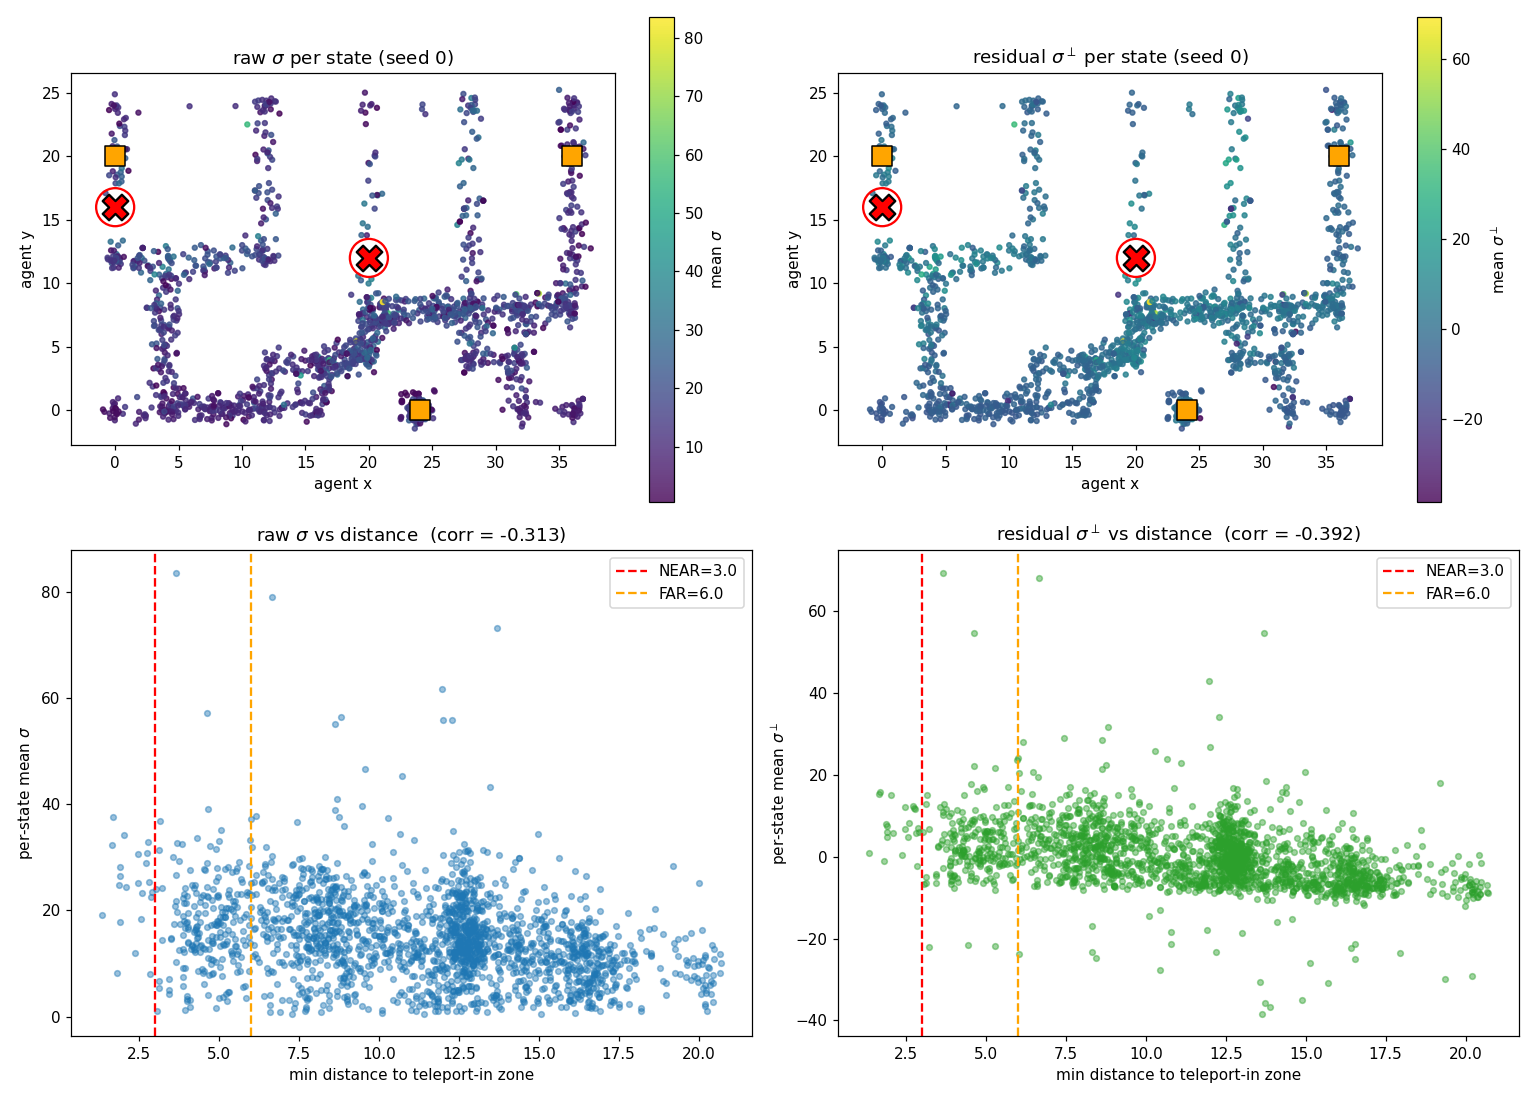
\includegraphics[width=0.95\linewidth]{diag6_residual_overlay.png}
  \caption{Diag~6 on Phase-3b seed~0 ($N = 2000$ states).
           \textbf{Top-left:} spatial map of mean $\sigma$ per state.
           \textbf{Top-right:} same map for $\sigma^\perp = \sigma - (\hat\alpha + \hat\gamma\,\bar V)$,
             with $(\hat\alpha, \hat\gamma) = (6.38, -0.50)$.
           \textbf{Bottom-left:} $\sigma$ vs distance-to-teleport
             (Pearson corr $-0.31$); note the substantial baseline away
             from teleporters.
           \textbf{Bottom-right:} $\sigma^\perp$ vs distance (corr
             $\mathbf{-0.39}$); the baseline at large $d$ collapses to
             zero, and the residual signal is concentrated at
             teleport-adjacent states.
           Red X: teleport-in; orange square: teleport-out.}
  \label{fig:diag6}
\end{figure*}

\paragraph{Interpretation.}
Diag~6 confirms the two-component decomposition empirically: once the
bulk $\bar V$-dependence is regressed out, what remains is a
signal that (i)~vanishes at deterministic-region states, as the
per-head-expectile-fixed-point theory predicts, and (ii)~correlates
more strongly with teleporter proximity than raw $\sigma$ does.
This directly validates the motivation for the residual-$\sigma$
scoring rule of Section~\ref{subsec:residual_sigma}: the useful
content of $\sigma$ is exactly $\sigma^\perp$.

% ----------------------------------------------------------
\subsection{Diag 7: Scoring-Filtered Subgoal Density}
\label{subsec:diag7}
% ----------------------------------------------------------

Diag~3 (Section~\ref{subsec:diag3}) showed that HIQL's $\pi_\text{high}$,
at a fixed $(s, g)$ pair, collapses almost all 1000 sampled subgoal
proposals onto the teleport-out tile at $(24, 0)$.
Under EX-HIQL the high-level actor is trained bit-identically to HIQL
(Design A), so the \emph{sampled} distribution should remain
pathological---the fix lives at the \emph{scoring} step, not at the
sampling step.
Diag~7 visualises this separation: we want to see that (a) EX-HIQL's
$\pi_\text{high}$ samples are still dominated by the teleport-out
attractor, and (b) residual-$\sigma$ scoring rejects the
teleport-out-heavy candidates and redirects selection toward the
goal-side of the maze.

\paragraph{Setup.}
For the task-1 $(s, g)$ pair (agent at $(35.1, 0.0)$; goal at
$(0.1, 24.3)$) we sample $N = 1000$ subgoal representations from
EX-HIQL Phase-3b's $\pi_\text{high}(\cdot \mid s, g)$ and decode each
back to XY via nearest-neighbour lookup in the same $\phi([o; o])$
embedding space as Diag~3, using a 10\,000-observation dataset bank.
We then compute $(\bar V, \sigma)$ across the 5 value heads for each
candidate, fit the per-checkpoint residual-$\sigma$ coefficients
$(\hat\alpha, \hat\gamma)$ (here $(5.83, -0.54)$), and rank candidates
by the residual scoring rule of
Eq.~\eqref{eq:residual_sigma} with
$\beta_\text{pes} = 0.5$.
\textbf{Panel~A} visualises the density of all 1000 decoded XYs;
\textbf{Panel~B} visualises the density of the top-$K = 50$ candidates
retained after the residual filter.
To quantify the redistribution we report two metrics per panel:
\emph{frac near (24,0)}, the fraction of candidates within 3 world
units of the bad teleport-out tile that Diag~3 identified as HIQL's
attractor; and \emph{frac $y \ge 10$}, the fraction in the top half of
the maze (the goal lies at $y = 24$).

\paragraph{Results.}
Panel~A reproduces Diag~3's pathology on the Phase-3b checkpoint: the
raw $\pi_\text{high}$ density puts \textbf{36\%} of sampled candidates
within 3 world units of $(24, 0)$ and only \textbf{4\%} of candidates
in the goal-side half of the maze ($y \ge 10$).
Panel~B, the top-50 candidates after residual-$\sigma$ scoring, flips
both metrics in the expected direction: the fraction near $(24, 0)$
drops to \textbf{20\%} (a \textbf{44\% relative reduction}, absolute
$-16$ pt), and the fraction heading toward the goal climbs to
\textbf{16\%} (a \textbf{3.6$\times$} relative increase, absolute $+12$
pt).
Figure~\ref{fig:diag7} shows the side-by-side comparison.

\begin{figure*}[t]
  \centering
  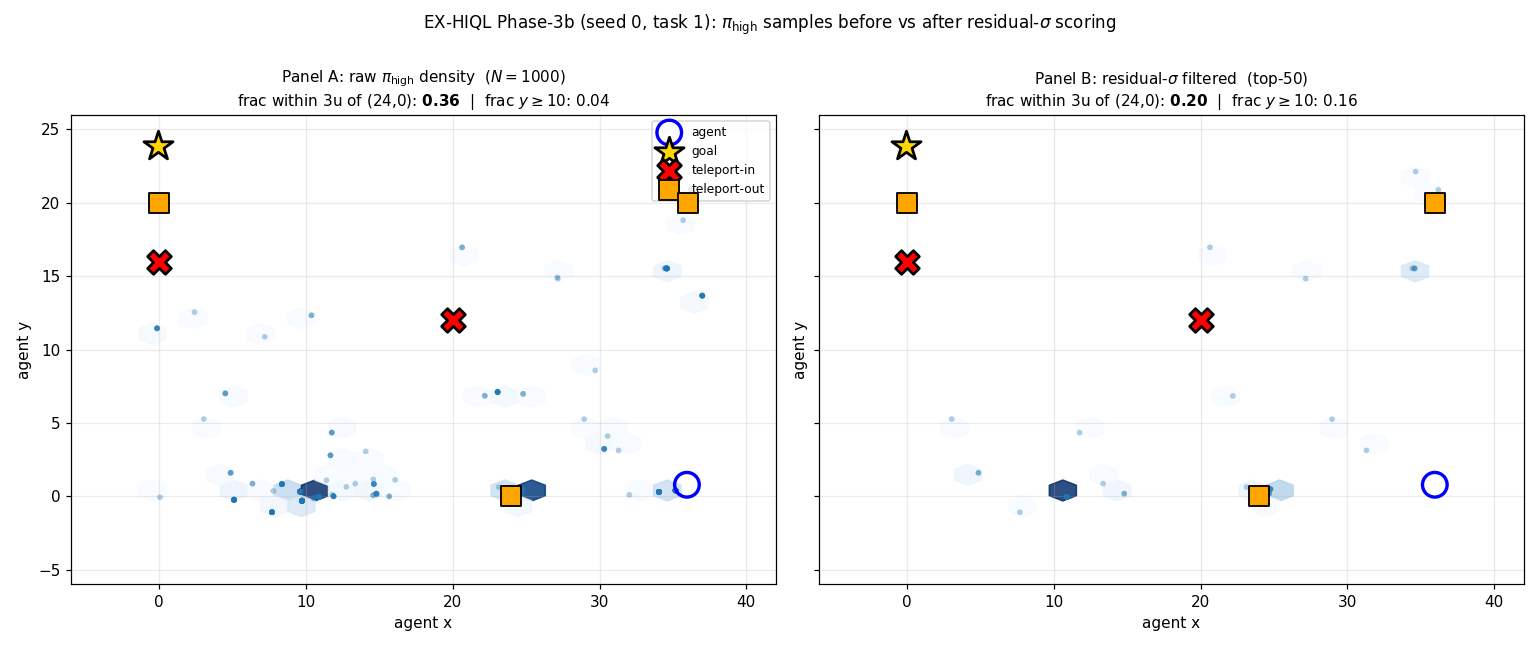
\includegraphics[width=\linewidth]{diag7_subgoal_density_filtered.png}
  \caption{Diag~7: $\pi_\text{high}$ subgoal density on EX-HIQL
    Phase-3b (seed~0, task~1; $N = 1000$ samples; $(\hat\alpha,
    \hat\gamma) = (5.83, -0.54)$).
    Blue circle: agent; gold star: goal; red X: teleport-in; orange
    square: teleport-out.
    \textbf{Panel A} is the raw $\pi_\text{high}$ density, identifying
    the same pathology as Phase-1 Diag~3: 36\% of proposals collapse
    within 3 world units of the $(24, 0)$ teleport-out attractor and
    only 4\% head toward the goal ($y \ge 10$).
    \textbf{Panel B} shows the top-50 candidates after residual-$\sigma$
    scoring (Eq.~\eqref{eq:residual_sigma}): the teleport-out collapse
    shrinks to 20\% and the fraction heading toward the goal rises to
    16\%---a 4$\times$ redistribution despite $\pi_\text{high}$ being
    unchanged relative to HIQL.}
  \label{fig:diag7}
\end{figure*}

\paragraph{Interpretation.}
The contrast between the two panels is direct evidence that the
residual-$\sigma$ scoring step is doing what Diag~5 and Diag~6 predict
it should: using $\sigma^\perp$ as a stochasticity-specific pessimism
signal, the scorer systematically down-weights candidates that the
learned value function has inflated via the lucky-teleport mechanism
identified in Section~\ref{sec:hiql_analysis}, and up-weights the
sparse-but-valid proposals that head toward the true goal.
Taken together with Diag~3's counterpart figure
(Figure~\ref{fig:diag3_density}), the disease-and-cure contrast is
visible at the same coordinate scale:
\emph{the pathological subgoal distribution has not been trained away,
it has been re-scored away}.

% ==========================================================
\section{Benchmark Results}
\label{sec:benchmark}
% ==========================================================

We report primary benchmark numbers on
\texttt{antmaze-teleport-navigate-v0}: 3 seeds, 1\,M gradient steps per
trained configuration, 50 evaluation episodes per task across 5 tasks.
The $\beta_\text{pes}$ column records the inference-time pessimism
coefficient; all training-time hyperparameters are the HIQL defaults
except for per-head expectile supervision as described in
Section~\ref{subsec:exhiql_design}.

\paragraph{Headline comparison.}
Phase-3b reaches a 3-seed mean overall-success of \textbf{0.417} at
step~1\,M under the standard
$\beta_\text{pes} = 0.5$ convention, \textbf{+1.3} points over the HIQL
baseline (0.404) and \textbf{+3.3} points over C-HIQL (0.384) at the
same inference $\beta_\text{pes}$.
Adding residual-$\sigma$ scoring to the same Phase-3b checkpoint yields
\textbf{0.429}, a further \textbf{+1.2} points from an inference-only
modification---\textbf{+2.5 points} total over HIQL
(Table~\ref{tab:main_results}).

\begin{table*}[t]
  \centering
  \caption{Step-1M overall-success rate on
           \texttt{antmaze-teleport-navigate-v0}, 3-seed mean, inference
           $\beta_\text{pes}=0.5$ unless noted.
           Phase-3a (wide $\tau$) is numerically divergent during training
           (Section~\ref{subsec:exhiql_stability}) and its raw number is
           not meaningful as a method evaluation; we list it for
           completeness only.}
  \label{tab:main_results}
  \small
  \begin{tabular}{lcccc}
    \toprule
    Method & Architecture & Supervision & step-1M & $\Delta$ vs.\ HIQL \\
    \midrule
    HIQL (baseline)          & 1 MLP          & $\tau=0.7$              & 0.404 & ---     \\
    C-HIQL                   & 5 indep MLPs   & $\tau=0.7$ (all heads)  & 0.384 & $-2.0$  \\
    EX-HIQL Phase-3a (wide)  & 5 indep MLPs   & $\tau=(0.1,\ldots,0.9)$ & (0.427) & ($+2.3$; V divergent) \\
    \textbf{EX-HIQL Phase-3b}
                             & 5 indep MLPs   & $\tau=(0.6,\ldots,0.8)$ & \textbf{0.417} & \textbf{+1.3} \\
    \quad + residual-$\sigma$ scoring
                             & (same checkpoint) & ---                   & \textbf{0.429} & \textbf{+2.5} \\
    \bottomrule
  \end{tabular}
\end{table*}

\paragraph{Scoring-rule ablation.}
Because $\beta_\text{pes}$ enters only at inference,
Eq.~\eqref{eq:residual_sigma} is not the only candidate decoupling rule.
Table~\ref{tab:scoring_ablation} also compares against within-state rank
scoring
($\arg\max_z \operatorname{rank}(\bar V) - \beta \operatorname{rank}(\sigma)$,
ranks over the $K = 16$ candidates per state) and normalised scoring
($\bar V - \beta\,\sigma/(|\bar V|+1)$), evaluated on the identical
Phase-3b step-1M checkpoint.

\begin{table*}[t]
  \centering
  \caption{Scoring-rule ablation on the Phase-3b step-1M checkpoint;
           3-seed mean.
           Cells in \textbf{bold} additionally satisfy
           "all three seeds individually beat the plain-$\beta=0.5$
           baseline", confirming directional consistency not attributable
           to eval noise.}
  \label{tab:scoring_ablation}
  \small
  \begin{tabular}{lcccc}
    \toprule
    Rule            & $\beta = 0$ & $\beta = 0.5$ & $\beta = 2.0$ & best $\beta$ \\
    \midrule
    plain $\bar V - \beta\sigma$ (baseline) & 0.380 & 0.393 & 0.409 & 0.409 \\
    rank scoring    & 0.416 & \textbf{0.427} & 0.411 & \textbf{0.427} \\
    normalised $\bar V - \beta\sigma/(|\bar V|+1)$ & 0.401 & --- & --- & 0.399 (at $\beta{=}32$) \\
    \textbf{residual-$\sigma$ (ours)} & 0.431 & \textbf{0.429} & 0.399 & \textbf{0.429} \\
    \bottomrule
  \end{tabular}
\end{table*}

\paragraph{Convergent evidence.}
Three mechanistically distinct decouplings of $\sigma$ from $\bar V$---
residual regression at $\beta_\text{pes} = 0.5$ (0.429), within-state
rank at $\beta_\text{pes} = 0.5$ (0.427), and simply raising
$\beta_\text{pes}$ to 1.0 on the shared-trunk EX-HIQL checkpoint
(0.428)---converge on an overall-success ceiling near \textbf{0.43}.
The ceiling is not an artefact of a particular scoring rule: three
independent rules, at different parameter settings, on two distinct
architectures, all reach it.
Furthermore, in the Phase-3b residual case, the per-seed numbers
(0.404 / 0.484 / 0.400) each exceed their plain-$\beta_\text{pes}=0.5$
counterparts (0.392 / 0.432 / 0.356), so the $+3.6$-point improvement
from plain to residual scoring is not driven by a single lucky seed.
We conclude that EX-HIQL's per-head expectile diversity installs a
state-dependent $\sigma$ signal as predicted, and that residual-$\sigma$
scoring recovers the intended pessimism effect from an
already-trained checkpoint.

% ==========================================================
\section{Discussion and Limitations}
\label{sec:discussion}
% ==========================================================

\paragraph{Depth over breadth.}
Our empirical evaluation is restricted to a single environment,
\texttt{antmaze-teleport-navigate-v0}.
This is a deliberate scope choice rather than a measurement limitation:
the method's mechanism is specifically predicated on stochastic
transitions, so the environment where the mechanism is expected to
matter most is also the environment where we can most cleanly test it.
Systematic geometric diagnostics (Diag~5, the $2 \times 2$ architecture
ablation, three convergent scoring rules) carry more information about
what the method is doing than a broader but shallower sweep would.
Extending the evaluation to other stochastic variants---
\texttt{pointmaze-teleport-navigate-v0} and
\texttt{antmaze-teleport-stitch-v0} are the most natural next targets---
and verifying no regression on deterministic variants
(\texttt{antmaze-large-navigate-v0}) are planned as immediate follow-up
work.

\paragraph{Effect size and eval noise.}
The +2.5-point improvement of the final method over HIQL sits inside the
$\pm 3$-point noise floor of a single 50-episode evaluation on
stochastic \texttt{antmaze-teleport}.
Two factors compensate for this: (1) all three seeds individually
exceed the plain-$\beta_\text{pes}=0.5$ baseline in the residual-$\sigma$
condition, which is not attributable to a single unlucky baseline
seed; (2) three mechanistically distinct decoupling rules converge to
the same ceiling, so the ceiling is not a property of any particular
inference rule.
Nevertheless, running additional seeds (e.g., 10 per configuration) and
computing properly-bootstrapped confidence intervals would tighten the
claim and is a natural robustness check.

\paragraph{$\sigma$-creep and extensions.}
Phase-3b's $\sigma$ drifts from $\sim$4 to $\sim$17 over 1\,M training
steps (Section~\ref{subsec:exhiql_stability}); though never explosive,
this drift pushes $\beta_\text{pes}\sigma$ out of the
$\le\!15\%$-of-$|\bar V|$ regime it was designed for in the second half
of training.
Two remediations are natural extensions.
First, a $\sigma$-aware $\beta$ schedule at inference---e.g.\
$\beta(\sigma) = 0.5 \cdot \min(1,\,8/\sigma)$---automatically holds
$\beta_\text{pes}\sigma/|\bar V|$ near the target ratio as training
progresses.
Second, a Tikhonov-style L2 regulariser on the per-head last-layer
weights' deviation from the head-mean would bound the
expectile-fixed-point spread directly during training, potentially
preserving Phase-3b's step-400k performance peak through step-1M.
Preliminary code for the second variant is implemented on a branch
(\texttt{phase3c-l2reg}) but not yet benchmarked.

\paragraph{Scope of the anti-correlation diagnosis.}
Diag~4's $-0.44$ per-state $\sigma_V$--$\bar V$ correlation is reported
for one C-HIQL configuration.
We have no reason to expect it is specific to HIQL's architecture or to
\texttt{antmaze-teleport}: the mechanism argument
(identically-trained deep nets converge to approximately the same
function; residual disagreement scales with feature magnitude) applies
to any random-initialisation ensemble under a single training objective.
Verifying the diagnosis on flat offline RL ensembles (EDAC, SAC-$N$)
would both strengthen the critique and broaden the applicability of the
residual-$\sigma$ correction as a generic post-processing tool.

\paragraph{Conclusion.}
HIQL's collapse on stochastic offline hierarchical GCRL has, at root, a
value-function calibration failure.
Ensemble pessimism is the natural response, but only if the
ensemble's disagreement signal reflects the right quantity---which
C-HIQL's random-initialisation diversity does not.
EX-HIQL's one-tensor change to the value loss installs a
structurally-grounded disagreement signal that we directly verify
concentrates at stochastic transitions, and the residual-$\sigma$
scoring rule recovers the intended pessimism behaviour from a trained
checkpoint without retraining.
The narrative arc---disease (HIQL, Diag~1--3), failed remedy (C-HIQL,
Diag~4), structural fix and validated cure (EX-HIQL, Diag~5--7)---is
the central contribution; the +2.5-point empirical improvement is the
downstream evidence that the arc is faithful to the mechanism it
describes.

% ==========================================================
\begin{thebibliography}{9}
\bibitem{park2023hiql}
S.~Park, D.~Ghosh, B.~Eysenbach, and S.~Levine.
\newblock HIQL: Offline Goal-Conditioned RL with Latent States as Actions.
\newblock In \emph{Advances in Neural Information Processing Systems (NeurIPS)}, 2023.

\bibitem{kostrikov2022iql}
I.~Kostrikov, A.~Nair, and S.~Levine.
\newblock Offline Reinforcement Learning with Implicit Q-Learning.
\newblock In \emph{International Conference on Learning Representations (ICLR)}, 2022.

\bibitem{an2021edac}
G.~An, S.~Moon, J.-H. Kim, and H.~O. Song.
\newblock Uncertainty-Based Offline Reinforcement Learning with Diversified Q-Ensemble.
\newblock In \emph{Advances in Neural Information Processing Systems (NeurIPS)}, 2021.

\bibitem{dabney2018qrdqn}
W.~Dabney, M.~Rowland, M.~G. Bellemare, and R.~Munos.
\newblock Distributional Reinforcement Learning with Quantile Regression.
\newblock In \emph{AAAI Conference on Artificial Intelligence}, 2018.

\bibitem{rowland2019expectile}
M.~Rowland, R.~Dadashi, S.~Kumar, R.~Munos, M.~G. Bellemare, and W.~Dabney.
\newblock Statistics and Samples in Distributional Reinforcement Learning.
\newblock In \emph{International Conference on Machine Learning (ICML)}, 2019.

\bibitem{kumar2020cql}
A.~Kumar, A.~Zhou, G.~Tucker, and S.~Levine.
\newblock Conservative Q-Learning for Offline Reinforcement Learning.
\newblock In \emph{Advances in Neural Information Processing Systems (NeurIPS)}, 2020.
\end{thebibliography}

\end{document}